\documentclass{scrartcl}
\usepackage[utf8]{inputenc}
\usepackage[german]{babel}
\usepackage{amsmath}
\usepackage{amssymb}
\usepackage{natbib}
\usepackage{graphicx}
\usepackage{float}
\usepackage{booktabs}
\usepackage[
  locale=DE,                   % deutsche Einstellungen
  separate-uncertainty=true,   % immer Fehler mit \pm
  per-mode=symbol-or-fraction, % / in inline math, fraction in display math
]{siunitx}
\floatplacement{figure}{htbp}
\floatplacement{table}{htbp}
\usepackage[
  section, % Floats innerhalb der Section halten
  below,   % unterhalb der Section aber auf der selben Seite ist ok
]{placeins}
\usepackage{subcaption}
\usepackage{xfrac}
\usepackage{enumitem}
\usepackage{dsfont}
\usepackage[
  labelfont=bf,        % Tabelle x: Abbildung y: ist jetzt fett
  font=small,          % Schrift etwas kleiner als Dokument
  width=0.9\textwidth, % maximale Breite einer Caption schmaler
]{caption}

\begin{document}
    \setlength{\parindent}{0em}

    \section*{Übungsblatt 9 -- Cerberus}

	%\section*{Aufgabe 1}

	\subsection*{Aufgabe 2}

\begin{figure}[h!]
\centering
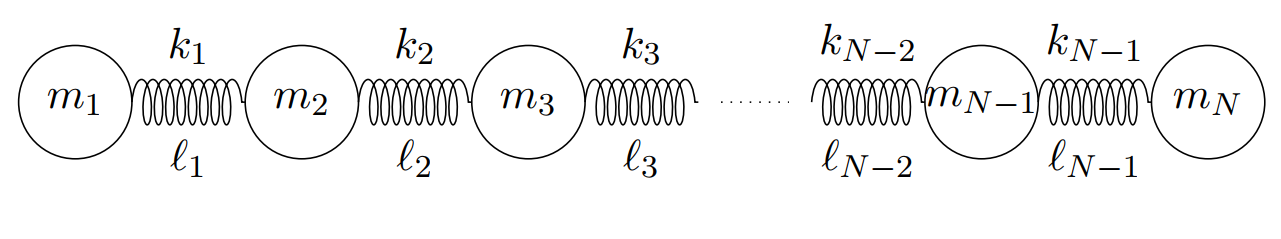
\includegraphics[width=0.8\textwidth]{content/images/Federn.png}
\label{fig:federn}
\end{figure}

\noindent In Abbildung \ref{fig:federn} ist eine Konfiguration von Federn der Ruhelänge $l_j$ mit Federkonstanten $k_j$ und Massen $m_i$ zu sehen, mit $i=1,...,N$ und $j = 1,...,N-1$. Des Weiteren gilt
\begin{align*}
m_i &= i\\
k_j &= N - j\\
l_j &= |5 - j| + 1
\end{align*}
Über den Kraftansatz für eine einzelne mit der Auslenkung aus der Ruhelage $x(t)$
\[
F = -kx(t) = m \ddot{x}(t) \Leftrightarrow {\frac{k}{m}}x + \ddot{x} = 0
\]
und auf Grund der Tatsache, dass nur die nächsten Nachbarn direkt über Federn verbunden sind lässt sich die Bewegung der $i$-ten Masse beschreiben als
\begin{align*}
\ddot{x_1} - \frac{k_1}{m_1}(x_2-x_1) &= 0\\
\ddot{x_i} - \frac{k_{i-1}}{m_i}(x_{i-1}-x_i)+\frac{k_i}{m_i}(x_{i+1}-x_i) &= 0\\
\ddot{x_N} - \frac{k_{N-1}}{m_N}(x_{N-1}-x_N) &= 0
\end{align*}
Mit dem Ansatz $x_i = \hat{x}_i\mathrm{e}^{i\omega t}$ lässt sich dieses $N\times N$-Gleichungssystem darstellen als
\begin{align*}
\begin{pmatrix}
\frac{k_1}{m_1}-\omega^2 & \frac{k_1}{m_1} & 0 & ... & 0 & 0\\
\frac{k_1}{m_2} & \frac{k_1+k_2}{m_2}- \omega^2 & \frac{k_2}{m_2} & 0 & ... & 0\\
0 & . & . & . & 0 & 0\\
. & 0 & . & . & . & 0\\
\end{pmatrix}\cdot\vec{\hat{x}} &= \vec{0}\\
\left(\begin{pmatrix}
\frac{k_1}{m_1} & \frac{k_1}{m_1} & 0 & ... & 0 & 0\\
\frac{k_1}{m_2} & \frac{k_1+k_2}{m_2} & \frac{k_2}{m_2} & 0 & ... & 0\\
0 & . & . & . & 0 & 0\\
. & 0 & . & . & . & 0\\
\end{pmatrix} - \omega^2\mathds{1}\right) \cdot\vec{\hat{x}} &= \vec{0}\\
\left(\mathbf{A}- \omega^2\mathds{1}\right) \cdot\vec{\hat{x}} &= \vec{0}
\end{align*}
Somit sind die Eigenwerte der Matrix $\mathbf{A}$, die beispielsweise über das Diagonalisieren der Tridiagonalmatrix bestimmt werden können, die Quadrate der Eigenfrequenzen $\omega$.
Für ein System mit $N=10$ Massen ergeben sich so die Eigenfrequenzen:
\begin{align*}
   \omega_1 = 3.95439\\
   \omega_2 = 2.62228\\
   \omega_3 = 1.95382\\
   \omega_4 = 1.51083\\
   \omega_5 = 1.17586\\
   \omega_6 = 0.901365\\
   \omega_7 = 0.663369\\
   \omega_8 = 1.23909\cdot 10^{-8}\\
   \omega_9 = 0.44762\\
   \omega_10 = 0.243446
\end{align*}
Die Frequenz $\omega_8$ sticht dabei auf Grund ihre niedrigen Potenz heraus. Der zugehörige Eigenwert der Matrix $\lambda_8 = 1.53534403\cdot 10^{-16}$ kommt vermutlich auf Grund von numerischer Instabilität und Rundungsfehlern zustande und sollte eigentlich bei $0$ liegen. Diese Vermutung wird auch dadurch unterstützt, dass bei Verwendung von \texttt{float}- statt \texttt{double}-Präzision der Wert dieser Eigenfrequenz ansteigt und bei $\omega_8 = 0.000241474$ liegt, während alle anderen Frequenzen unverändert bleiben.
%☺☻

	%\subsection*{Aufgabe 3}

\end{document}
